\documentclass[10pt,letterpaper]{article}\usepackage[]{graphicx}\usepackage[]{color}
%% maxwidth is the original width if it is less than linewidth
%% otherwise use linewidth (to make sure the graphics do not exceed the margin)
\makeatletter
\def\maxwidth{ %
  \ifdim\Gin@nat@width>\linewidth
    \linewidth
  \else
    \Gin@nat@width
  \fi
}
\makeatother

\definecolor{fgcolor}{rgb}{0.345, 0.345, 0.345}
\newcommand{\hlnum}[1]{\textcolor[rgb]{0.686,0.059,0.569}{#1}}%
\newcommand{\hlstr}[1]{\textcolor[rgb]{0.192,0.494,0.8}{#1}}%
\newcommand{\hlcom}[1]{\textcolor[rgb]{0.678,0.584,0.686}{\textit{#1}}}%
\newcommand{\hlopt}[1]{\textcolor[rgb]{0,0,0}{#1}}%
\newcommand{\hlstd}[1]{\textcolor[rgb]{0.345,0.345,0.345}{#1}}%
\newcommand{\hlkwa}[1]{\textcolor[rgb]{0.161,0.373,0.58}{\textbf{#1}}}%
\newcommand{\hlkwb}[1]{\textcolor[rgb]{0.69,0.353,0.396}{#1}}%
\newcommand{\hlkwc}[1]{\textcolor[rgb]{0.333,0.667,0.333}{#1}}%
\newcommand{\hlkwd}[1]{\textcolor[rgb]{0.737,0.353,0.396}{\textbf{#1}}}%
\let\hlipl\hlkwb

\usepackage{framed}
\makeatletter
\newenvironment{kframe}{%
 \def\at@end@of@kframe{}%
 \ifinner\ifhmode%
  \def\at@end@of@kframe{\end{minipage}}%
  \begin{minipage}{\columnwidth}%
 \fi\fi%
 \def\FrameCommand##1{\hskip\@totalleftmargin \hskip-\fboxsep
 \colorbox{shadecolor}{##1}\hskip-\fboxsep
     % There is no \\@totalrightmargin, so:
     \hskip-\linewidth \hskip-\@totalleftmargin \hskip\columnwidth}%
 \MakeFramed {\advance\hsize-\width
   \@totalleftmargin\z@ \linewidth\hsize
   \@setminipage}}%
 {\par\unskip\endMakeFramed%
 \at@end@of@kframe}
\makeatother

\definecolor{shadecolor}{rgb}{.97, .97, .97}
\definecolor{messagecolor}{rgb}{0, 0, 0}
\definecolor{warningcolor}{rgb}{1, 0, 1}
\definecolor{errorcolor}{rgb}{1, 0, 0}
\newenvironment{knitrout}{}{} % an empty environment to be redefined in TeX

\usepackage{alltt}
\usepackage[top=0.85in,left=1.75in,footskip=0.75in]{geometry}

% amsmath and amssymb packages, useful for mathematical formulas and symbols
\usepackage{amsmath,amssymb}

% Use adjustwidth environment to exceed column width (see example table in text)
\usepackage{changepage}

% Use Unicode characters when possible
\usepackage[utf8x]{inputenc}

% textcomp package and marvosym package for additional characters
\usepackage{textcomp,marvosym}

% cite package, to clean up citations in the main text. Do not remove.
\usepackage{cite}

% Use nameref to cite supporting information files (see Supporting Information section for more info)
\usepackage{nameref,hyperref}

% line numbers
\usepackage[right]{lineno}

% ligatures disabled
\usepackage{microtype}
\DisableLigatures[f]{encoding = *, family = * }

% color can be used to apply background shading to table cells only
\usepackage[table]{xcolor}

% array package and thick rules for tables
\usepackage{array}

% bold math symbols package
\usepackage{bm}

% nice figures and captions
\usepackage{graphicx}

% diagrams or complicated equations
\usepackage{tikz}

% vertical and horizontal dashed lines
\usepackage{arydshln}

%\usepackage{setspace}

%\usepackage{floatflt}
%\usepackage{nonfloat}
\usepackage{float}
\usepackage{wrapfig}

%\renewcommand{\arraystretch}{1.2}
%\setlength{\tabcolsep}{12pt}

% create "+" rule type for thick vertical lines
\newcolumntype{+}{!{\vrule width 2pt}}

% create \thickcline for thick horizontal lines of variable length
\newlength\savedwidth
\newcommand\thickcline[1]{%
  \noalign{\global\savedwidth\arrayrulewidth\global\arrayrulewidth 2pt}%
  \cline{#1}%
  \noalign{\vskip\arrayrulewidth}%
  \noalign{\global\arrayrulewidth\savedwidth}%
}

% \thickhline command for thick horizontal lines that span the table
\newcommand\thickhline{\noalign{\global\savedwidth\arrayrulewidth\global\arrayrulewidth 2pt}%
\hline
\noalign{\global\arrayrulewidth\savedwidth}}


% Remove comment for double spacing
%\usepackage{setspace} 
%\doublespacing

% Text layout
% \raggedright
\setlength{\parindent}{0.5cm}
\textwidth 5.25in 
\textheight 8.75in

% Bold the 'Figure #' in the caption and separate it from the title/caption with a period
% Captions will be left justified
\usepackage[aboveskip=1pt,labelfont=bf,labelsep=period,justification=raggedright,singlelinecheck=off]{caption}
\renewcommand{\figurename}{Fig}

% Use the PLoS provided BiBTeX style
%\bibliographystyle{plos2015}


% Remove brackets from numbering in List of References
\makeatletter
\renewcommand{\@biblabel}[1]{\quad#1.}
\makeatother

% define theorem and definition environments commands
\newtheorem{theorem}{Theorem}[section]
\newtheorem{definition}{Definition}[section]

% Header and Footer with logo
\usepackage{lastpage,fancyhdr,graphicx}
\usepackage{epstopdf}
%\pagestyle{myheadings}
\pagestyle{fancy}
\fancyhf{}
%\setlength{\headheight}{27.023pt}
%\lhead{\includegraphics[width=2.0in]{PLOS-submission.eps}}
\rfoot{\thepage/\pageref{LastPage}}
\renewcommand{\headrulewidth}{0pt}
\renewcommand{\footrule}{\hrule height 2pt \vspace{2mm}}
\fancyheadoffset[L]{2.25in}
% \fancyfootoffset[L]{1.25in}
\lfoot{\today}


\restylefloat{figure}


%% Include all macros below

\newcommand{\lorem}{{\bf LOREM}}
\newcommand{\ipsum}{{\bf IPSUM}}

\def\lf{\left\lfloor}   
\def\rf{\right\rfloor}

\def\ri{R_i}
\def\rj{R_j}
\def\kmi{k_{M_i}}
\def\khi{k_{H_i}}
\def\hji{H_{j_i}}
\def\ma{\overline{M}_a}
\def\ha{\overline{H}_a}
\def\mnu{M_\nu}
\def\hnu{H_\nu}
\def\myd{\text{diff}}
\def\ka{\bar{k}_\alpha}
\def\mji{M_{j_i}}

%% END MACROS SECTION
\IfFileExists{upquote.sty}{\usepackage{upquote}}{}
\begin{document}
\vspace*{0.2in}

% Title must be 250 characters or less.
% \begin{flushleft}
{\Large
\textbf\newline{Novel metrics and application of nearest-neighbor feature selection for creating resting-state fMRI brain atlases} % Please use "sentence case" for title and headings (capitalize only the first word in a title (or heading), the first word in a subtitle (or subheading), and any proper nouns).
}
%\newline
% Insert author names, affiliations and corresponding author email (do not include titles, positions, or degrees).
\begin{center}
  \begin{tabular}{l}
  Bryan A. Dawkins$^{\text{1}}$, Trang T. Le$^{\text{2}}$, Alejandro A. Hernandez$^{\text{1}}$, and Brett A. McKinney$^{\text{1,3,}*}$ \\
  $^{\text{1}}$Department of Mathematics, University of Tulsa, Tulsa, OK 74104, USA \\
  $^{\text{2}}$Department of Biostatistics, Epidemiology and Informatics, University of \\
  \hphantom{2}Pennsylvania, Philadelphia, PA 19104 \\
  $^{\text{3}}$Tandy School of Computer Science, University of Tulsa, Tulsa, OK 74104, USA.
  \end{tabular}
\end{center}


% \end{flushleft}
% Please keep the abstract below 300 words
\section*{Abstract}
Resting-state functional connectivity MRI (rs-fMRI) data consists of correlation matrices, where correlations are computed between the time series from brain Regions of Interest (ROIs). There are many different parcellations of the human brain into collections of ROIs. These parcellations, or atlases, can be used in case-control studies in order to understand and accurately classify subject phenotypes. We present new metrics for nearest-neighbor distance-based feature selection at the ROI level. Using our new metrics, we apply a novel nearest-neighbor feature selection algorithm to calculate relative importance of ROIs in two existing brain atlases. We use integer programming to derive a mapping between brain atlases to determine spatially similar ROIs. With ROI importance scores and spatial similarity between atlases, we create a new brain parcellation that combines aspects of both brain atlases.
\linenumbers

%\doublespacing
\section{Background}
Resting-state fMRI data exists in high dimensions and has many sources of noise, such as physiological or motion related~\cite{caballero2017}. Feature selection is typically done with the purpose of determining brain regions of interest (ROIs) that accurately discriminate between cases and controls in order to understand a particular phenotype. The data consists of pairwise ROI-ROI correlations, where each ROI is a time series measuring brain activity in a particular region or regions of the brain while a subject is not performing a task. A typical data set consists of $m$ subject-specific correlation matrices of dimension $p \times p$, where the pairwise correlations are computed between $p$ ROIs from a brain atlas. Nearest-neighbor distance-based feature selection in rs-fMRI data has been performed using the private evaporative cooling method, which used pairwise ROI-ROI correlations as predictors of a particular phenotype. However, nearest-neighbor feature selection algorithms have not been applied at the ROI level to assess the relative importance of ROIs for a given phenotype. To address this, we have previously proposed a new distance metric that allows us to compute the importance of individual ROIs using a nearest-neighbor distance-based approach. We use this new distance metric with a novel nearest-neighbor feature selection algorithm called Nearest-neighbor Projected Distance Regression (NPDR) in order to compute ROI importance and the corresponding pseudo P values~\cite{npdr}. Our analysis is done on subject rs-fMRI correlation matrices generated by two well known brain atlases~\cite{power2011,shen2013}. 

In order to make spatial comparisons between any pair of brain atlases, we first compute a distance matrix containing all pairwise distances between the different collections of atlas ROIs. Distances are defined based on a set dissimilarity metric that accounts for differences in voxel collections between pairs of ROIs. In a particular coordinate system, voxels have well defined three-dimensional locations in a given brain atlas. As long as two different atlases are in the same coordinate system, we can compare voxel membership between opposing atlas ROIs. We use an integer program that defines the standard Assignment Problem (AP) to find the one-to-one mapping between the two sets of atlas ROIs~\cite{pentico2007}. The collection of all mapped ROIs gives the closest spatial analogy between the two atlases, which tells us the closest relationship between the two sets of ROIs from different atlases. The collection of unmapped ROIs gives an indication of spatial uniqueness in the two atlases, respectively. All ROIs can be further mapped to a well defined anatomical region of the brain, which allows us to point out potential targets for better understanding the phenotype of interest.

Our spatial mapping between atlases and relative importance scores for ROIs in each respective atlas provides a way to combine relevant and distinct aspects of each brain atlas into a new parcellation. This new atlas includes important ROIs that are in the optimal one-to-one mapping from the solution to the assignment problem and any important unmapped ROIs from each atlas. Spatial overlap and attribute importance can serve as a useful tool for other researchers to compare, contrast, and combine two atlases. In particular, our results show how one might choose either of the two atlases to study the phenotype of interest we are considering in this work.

\section{Methods}
In this section, we first describe real rs-fMRI data generated from healthy controls (HC) and subjects with major depressive disorder (MDD), eating disorder (ED), substance abuse (SA), or anxiety disorder (AD). Using integer programming, we then derive a one-to-one mapping between the ROIs in two brain atlases used to generate the real data mentioned previously. Finally, we use our new distance metric for rs-fMRI data, along with NPDR, to compute importance scores for ROIs in each atlas from the real data.

\subsection{Real rs-fMRI data}
% need to get with Rayus to discuss the details on what the data is, how it was processed,
% more demographics info for subjects, and anything else that might be important
This is where we describe the LIBR data.

\subsection{Spatial overlap between brain atlases}
Let $R_A$ and $R_B$ represent regions of interest (ROIs) in atlases $A$ and $B$, respectively. We assume that atlases $A$ and $B$ are in the same coordinate space. Since $R_A$ and $R_B$ are just collections of voxels that have well defined three-dimensional coordinates within an atlas, the spatial overlap between $R_A$ and $R_B$ can be defined as the set intersection between the two ROIs. Spatial dissimilarity between $R_A$ and $R_B$ can be computed with the Jaccard metric, which is given by the following
%
\begin{equation}\label{eq:jaccard}
\text{d}^\text{J}(R_A,R_B) = \frac{|R_A \cup R_B - R_A \cap R_B|}{|R_A \cup R_B|},
\end{equation}
%
where the ($-$) sign denotes set complement and $|\cdot|$ represents set cardinality. If the intersection $R_A \cap R_B$ is empty, then the two ROIs do not share any voxels and the Jaccard distance (Eq.~\ref{eq:jaccard}) between them is 1. On the other hand, the Jaccard distance is 0 if the union $R_A \cup R_B$ and intersection $R_A \cap R_B$ are the same sets, which means the two ROIs have exactly the same voxels. All other possible Jaccard distances between $R_A$ and $R_B$ are strictly within $(0,1)$. Hence, the Jaccard metric is contained within $[0,1]$. The reason for division by $|R_A \cup R_B|$ in the denominator of the Jaccard metric (Eq.~\ref{eq:jaccard}) is specifically to normalized the distance to be within $[0,1]$. Otherwise, this distance between two ROIs would be affected by the cardinalities of $R_A$ and $R_B$, respectively. The Jaccard metric is intuitive in this context because ROIs are not just points in space, but rather they can have irregular three-dimensional shapes. Therefore, a Euclidean metric that gives the straight-line distance between two points does not necessarily indicate `closeness' between two ROIs. It is possible to compute the Euclidean distance between the centroids of two ROIs, but the ROIs may not share many voxels due to their potentially irregular shapes. Therefore, it is more informative to use a distance metric that uses set operations like the Jaccard metric (Eq.~\ref{eq:jaccard}). We show an example (Fig.~\ref{fig:jaccard}) of the Jaccard distance between ROIs $R_A$ and $R_B$ that contain $n_1$ and $n_2$ voxels, respectively. 

\vspace{0.25cm}

% trim=left botm right top
%\begin{figure}[h!]\label{fig:jaccard}
	{\centering
	\begin{minipage}[c]{0.55\textwidth}
	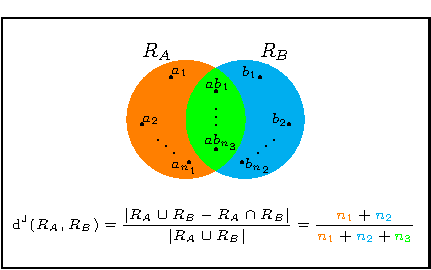
\includegraphics[width=1\textwidth,clip,trim=0cm 0cm 0cm 0.26cm]{venn_diagram.pdf}
	\end{minipage}\hfill
	\begin{minipage}[c]{0.43\textwidth}
	\captionsetup{type=figure}\captionof{figure}{Example computation of Jaccard distance between ROIs $R_A$ and $R_B$ from two atlases $A$ and $B$, respectively. There are $n_1$, $n_2$, $n_3$ voxels in $R_A$ only, $R_B$ only, and both $R_A$ and $R_B$, respectively. The numerator gives the number of voxels unique to $R_A$ ($n_1$) plus the number of voxels unique to $R_B$ ($n_2$). The denominator contains the total number of voxels in $R_A$ or $R_B$.}\label{fig:jaccard}
	\end{minipage}}
%\end{figure}

\vspace{0.25cm}

Each ROI in atlas $A$ may overlap many different ROIs in atlas $B$. On the other hand, some ROIs in $A$ may not overlap any ROIs in $B$. Furthermore, it is likely that $A$ and $B$ contain different numbers of ROIs. If we want to compute a minimum distance one-to-one mapping between the atlases, it is possible that some ROIs in $A$ will not have a mapped partner in $B$. 

\subsection{Relative importance of ROIs}

\section{Results}

\subsection{New brain atlas}

\section{Discussion}

\bibliographystyle{unsrt}
\bibliography{BoD}   % name of bib file
\end{document}
